\chapter{Highnoon}
\noindent Karta udalosti sa odhaľuje od druhého ťahu šerifa ešte pred jeho vlastným ťahom a jej efekt platí, kým ju neprekryje ďalšia udalosť. Formulácia „na začiatku ťahu“ znamená ešte pred akoukoľvek inou akciou hráča.
\begin{figure}[!h]
    \centering
    \begin{minipage}[t]{\minipageSize}\centering
      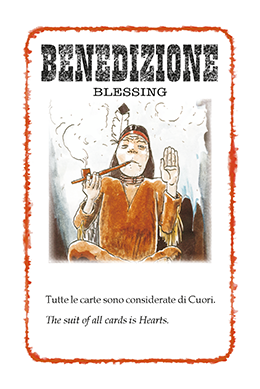
\includegraphics[width=\cardSize\linewidth]{highnoon/05_benedizione.png}
      \caption[Benedizione]{Všetky karty sú považované za srdcové.}
    \end{minipage}
    \hfill
    \begin{minipage}[t]{\minipageSize}\centering
      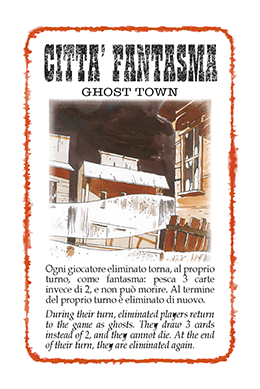
\includegraphics[width=\cardSize\linewidth]{highnoon/05_cittafantasma.png}
      \caption[Città Fantasma]{Vyradení hráči sa vo svojom ťahu vracajú ako duchovia. Vo fáze 1 si potiahnú 3 karty a môžu pri tom používať svoje schopnosti, napr. Pedro Ramiréz; Bill No Face pri návrate ako duch vstupuje s 5 kartami a Pixie Pete s 3 kartami. Na konci ťahu sú opäť vyradení, odhodia svoje karty a ak je Vulture Sam v hre, vezme si ich. Každý odchod ducha z hry spúšťa schopnosti Grega Diggera a Herba Huntera. Ak hra skončí počas ťahu ducha, vyhodnotí sa, ako keby bol stále v hre.}
    \end{minipage}
    \hfill
    \begin{minipage}[t]{\minipageSize}\centering
      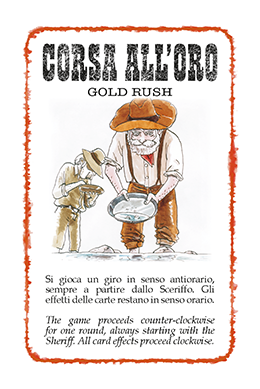
\includegraphics[width=\cardSize\linewidth]{highnoon/05_corsaalloro.png}
      \caption[Corsa all'Oro]{Hra prebieha proti smeru hodinových ručičiek, začínajúc šerifom. Všetky efekty kariet pokračujú v pôvodnom smere.}
    \end{minipage}
    \hfill
    \begin{minipage}[t]{\minipageSize}\centering
      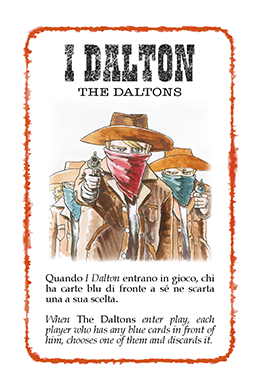
\includegraphics[width=\cardSize\linewidth]{highnoon/05_idalton.png}
      \caption[I Dalton]{Každý hráč, ktorý má pred sebou modré karty, musí jednu z nich odhodiť.}
    \end{minipage}
\end{figure}

\begin{figure}[!h]
    \centering
    \begin{minipage}[t]{\minipageSize}\centering
      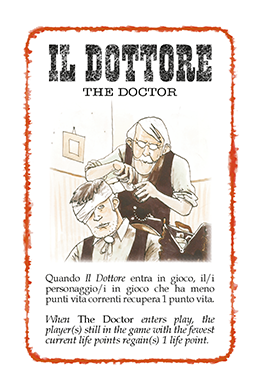
\includegraphics[width=\cardSize\linewidth]{highnoon/05_ildottore.png}
      \caption[Il Dottore]{Hráči s najmenším počtom životov si obnovia 1 život.}
    \end{minipage}
    \hfill
    \begin{minipage}[t]{\minipageSize}\centering
      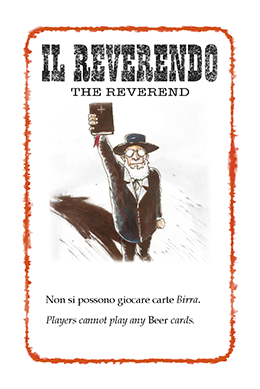
\includegraphics[width=\cardSize\linewidth]{highnoon/05_ilreverendo.png}
      \caption[Il Reverendo]{Hráči nemôžu hrať kartu Pivo. Zákaz sa vzťahuje na konkrétnu kartu Pivo, nie automaticky na každý efekt Pivo.}
    \end{minipage}
    \hfill
    \begin{minipage}[t]{\minipageSize}\centering
      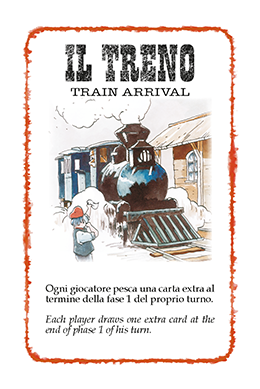
\includegraphics[width=\cardSize\linewidth]{highnoon/05_iltreno.png}
      \caption[Il Treno]{Každý hráč si na konci fázy 1 doberie 1 kartu navyše. Kid Carlson schopnosť v tomto prípade nemá žiadny efekt.}
    \end{minipage}
    \hfill
    \begin{minipage}[t]{\minipageSize}\centering
      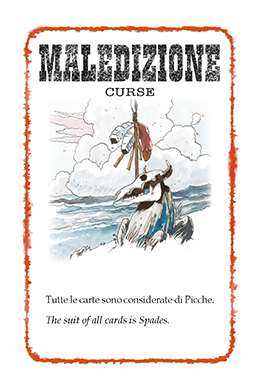
\includegraphics[width=\cardSize\linewidth]{highnoon/05_maledizione.png}
      \caption[Maledizione]{Všetky karty sú považované za pikové.}
    \end{minipage}
\end{figure}

\begin{figure}[!h]
    \centering
    \begin{minipage}[t]{\minipageSize}\centering
      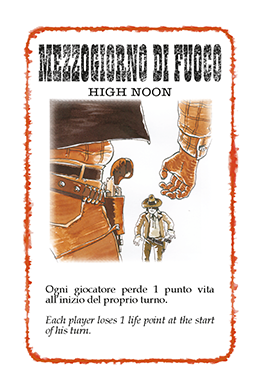
\includegraphics[width=\cardSize\linewidth]{highnoon/05_mezzogiornodifuoco.png}
      \caption[Mezzogiorno di Fuoco]{Každý hráč na začiatku ťahu stratí 1 život.}
    \end{minipage}
    \hfill
    \begin{minipage}[t]{\minipageSize}\centering
      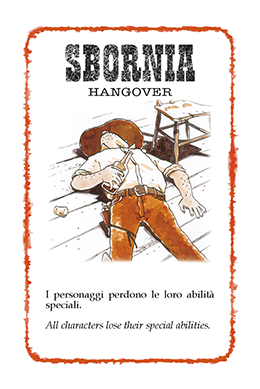
\includegraphics[width=\cardSize\linewidth]{highnoon/05_sbornia.png}
      \caption[Sbornia]{Všetky postavy strácajú svoje špeciálne schopnosti.}
    \end{minipage}
    \hfill
    \begin{minipage}[t]{\minipageSize}\centering
      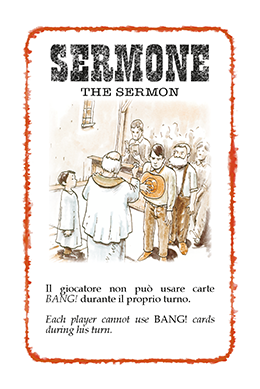
\includegraphics[width=\cardSize\linewidth]{highnoon/05_sermone.png}
      \caption[Sermone]{Hráči nesmú hrať karty BANG! počas svojho ťahu. Nemôžu sa používať ani počas duelu a ani postavy ako Calamity Janet etc. .\cite{HighNoon}}
    \end{minipage}
    \hfill
    \begin{minipage}[t]{\minipageSize}\centering
      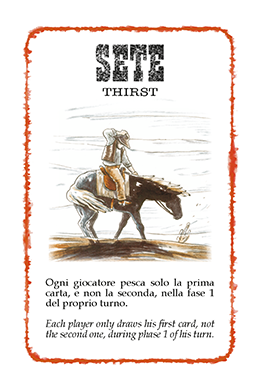
\includegraphics[width=\cardSize\linewidth]{highnoon/05_sete.png}
      \caption[Sete]{Každý hráč si potiahne o -1 kartu ako normálne vo fáze 1. Kid Carlson sa aj tak pozrie na tri vrchné karty no zoberie si len jednu.}
    \end{minipage}
\end{figure}

\begin{figure}[!h]
    \begin{minipage}[t]{\minipageSize}\centering
      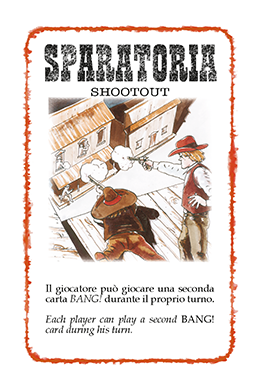
\includegraphics[width=\cardSize\linewidth]{highnoon/05_sparatoria.png}
      \caption[Sparatoria]{Každý hráč môže počas ťahu zahrať dve karty BANG!}
    \end{minipage}
    \hfill
    \begin{minipage}[t]{0.22\linewidth}\centering
      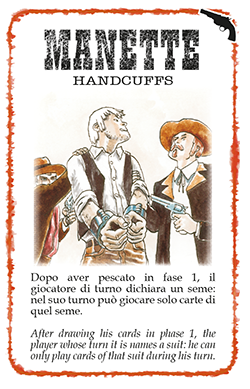
\includegraphics[width=\cardSize\linewidth]{highnoon/bonus-Manette.png}
      \caption[Manette]{Po potiahnutí kariet si hráč určí farbu. Počas ťahu môže hrať iba karty tejto farby. Efekt platí len počas kola hráča.}
    \end{minipage}
    \hfill
    \begin{minipage}[t]{0.22\linewidth}\centering
      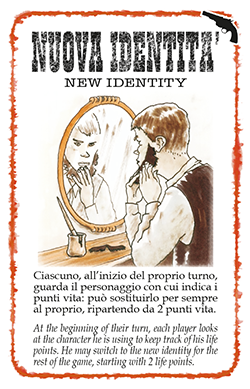
\includegraphics[width=\cardSize\linewidth]{highnoon/bonus-NuovaIdentita.png}
      \caption[Nuova Identita]{Na začiatku svojho ťahu môže hráč vymeniť svoju postavu za svoju kartu životov, ale začína len s 2 životmi.}
    \end{minipage}
     \hfill
    \begin{minipage}[t]{\minipageSize}\centering
    \end{minipage}
\end{figure}
